%Folgende Zeile aktivieren und als SVN property "svn:keywords" auf "Id" setzen, um SVN Versionsinformationen im Dokument zu erhalten
%\svnInfo $Id: einleitung.tex 60 2012-01-26 15:56:06Z koppor $ 

\chapter{Problemstellung}
Eine Möglichkeit der Verfälschung der erkannten Objekte zu begegnen ist die Ersetzung bzw. Approximierung dieser durch einfachere Objekte (z.B. Zylinder, Kugel oder Quader). Im Rahmen der Fachstudie sollten deshalb Algorithmen ausfindig gemacht werden mit denen die genannten Objekte innerhalb der Bilddaten erkannt werden können. Anhand einfacher Teststrukturen sollte eine Auswahl vielversprechender Algorithmen getestet und miteinander verglichen werden. Die Ergebnisse wurden protokolliert und bewertet.

\begin{figure}[H]
  \begin{center}
    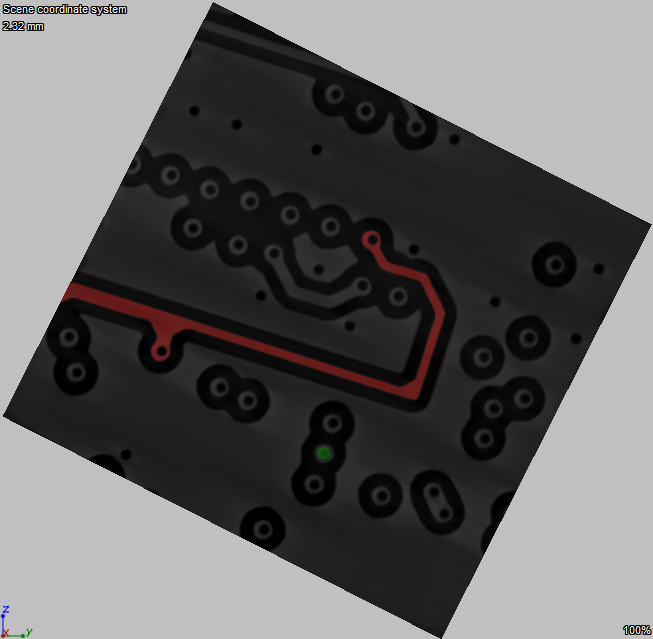
\includegraphics[width=0.5\textwidth]{zuerkennende.png}
    \caption{Typischer 2D-Slice mit Leiterbahnen (rot) und Bohrpunkten (grün)}
    \label{fig:zuerkennende1}
  \end{center}
\end{figure}

